%%%%%%%%%%%%%%%%%%%%%%%%%%%%%%%%%%%%%%%%%
% NIWeek 2014 Poster by T. Reveyrand
% www.microwave.fr
% http://www.microwave.fr/LaTeX.html
% ---------------------------------------
% 
% Original template created by:
% Brian Amberg (baposter@brian-amberg.de)
%
% This template has been downloaded from:
% http://www.LaTeXTemplates.com
%
% License:
% CC BY-NC-SA 3.0 (http://creativecommons.org/licenses/by-nc-sa/3.0/)
%
%%%%%%%%%%%%%%%%%%%%%%%%%%%%%%%%%%%%%%%%%

%----------------------------------------------------------------------------------------
%	PACKAGES AND OTHER DOCUMENT CONFIGURATIONS
%----------------------------------------------------------------------------------------

\documentclass[a0paper,portrait]{baposter}

\usepackage[font=small,labelfont=bf]{caption} % Required for specifying captions to tables and figures
\usepackage{booktabs} % Horizontal rules in tables
\usepackage{relsize} % Used for making text smaller in some places

\usepackage{amsmath,amsfonts,amssymb,amsthm} % Math packages
\usepackage{eqparbox}
\usepackage{ctex} % 支持中文,需要XeLeTex编译
\usepackage{textcomp}

%\usepackage{caption}
\usepackage{subfigure}

\usepackage{lmodern}

\graphicspath{{figures/}} % Directory in which figures are stored

 \definecolor{bordercol}{RGB}{40,40,40} % Border color of content boxes
 \definecolor{headercol1}{RGB}{186,215,230} % Background color for the header in the content boxes (left side)
 \definecolor{headercol2}{RGB}{120,120,120} % Background color for the header in the content boxes (right side)
 \definecolor{headerfontcol}{RGB}{0,0,0} % Text color for the header text in the content boxes
 \definecolor{boxcolor}{RGB}{255,255,255} % Background color for the content in the content boxes

\def\ie{\emph{i.e.}}
\def\eg{\emph{e.g.}}
\def\resp{\emph{resp.}}
\def\etal{\emph{et al.}}
\def\wrt{\emph{w.r.t.}}
\def\aka{\emph{a.k.a.}}
\def\vs{\emph{v.s.}}

\def\tr{\mbox{tr}}

\def\1{\mathbf{1}}
\def\0{\mathbf{0}}

\def\x{\mathbf{x}}
\def\y{\mathbf{y}}
\def\z{\mathbf{z}}
\def\p{\mathbf{p}}
\def\u{\mathbf{u}}
\def\v{\mathbf{v}}
\def\w{\mathbf{w}}

\def\hy{\hat{y}}
\def\hby{\hat{\mathbf{y}}}

\def\tbx{\tilde{\mathbf{x}}}

\def\bTheta{\mathbf{\Theta}}

\def\P{\mathbf{P}}
\def\Q{\mathbf{Q}}
\def\M{\mathbf{M}}
\def\T{\mathbf{T}}
\def\I{\mathbf{I}}
\def\K{\mathbf{K}}
\def\X{\mathbf{X}}
\def\Y{\mathbf{Y}}
\def\A{\mathbf{A}}
\def\B{\mathbf{B}}
\def\C{\mathbf{C}}

\def\hbT{\hat{\mathbf{T}}}

\def\tM{\tilde{M}}
\def\tbM{\tilde{\mathbf{M}}}
\def\tbX{\tilde{\mathbf{X}}}

\def\cE{{\mathcal E}}
\def\cD{{\mathcal D}}
\def\cI{{\mathcal I}}
\def\cT{{\mathcal T}}
\def\cL{{\mathcal L}}
\def\cX{{\mathcal X}}
\def\cY{{\mathcal Y}}

\def\bcI{\bar{\mathcal I}}

\def\bE{{\mathbb E}}

\def\bmu{\mbox{\boldmath $\mu$}}
\def\bxi{\mbox{\boldmath $\xi$}}
\def\hbX{\hat{\mathbf{X}}}
\def\hbx{\hat{\mathbf{x}}}

\usepackage{color}
\def\red{\textcolor{red}}
\def\blue{\textcolor{blue}}
\def\green{\textcolor{green}}
\def\melon{\textcolor{melon}}
\def\paper{\textcolor{blue}}

\def\diag{\mbox{diag}}

\def\name{OTOS}
\def\namea{OTOS-$\alpha$}
\def\nameb{OTOS-$\beta$}

\begin{document}

\background{ % Set the background to an image (background.pdf),如果不需要背景,就是默认的白色背景
	%\begin{tikzpicture}[remember picture,overlay]
	%\draw (current page.north west)+(-2em,2em) node[anchor=north west]
	%{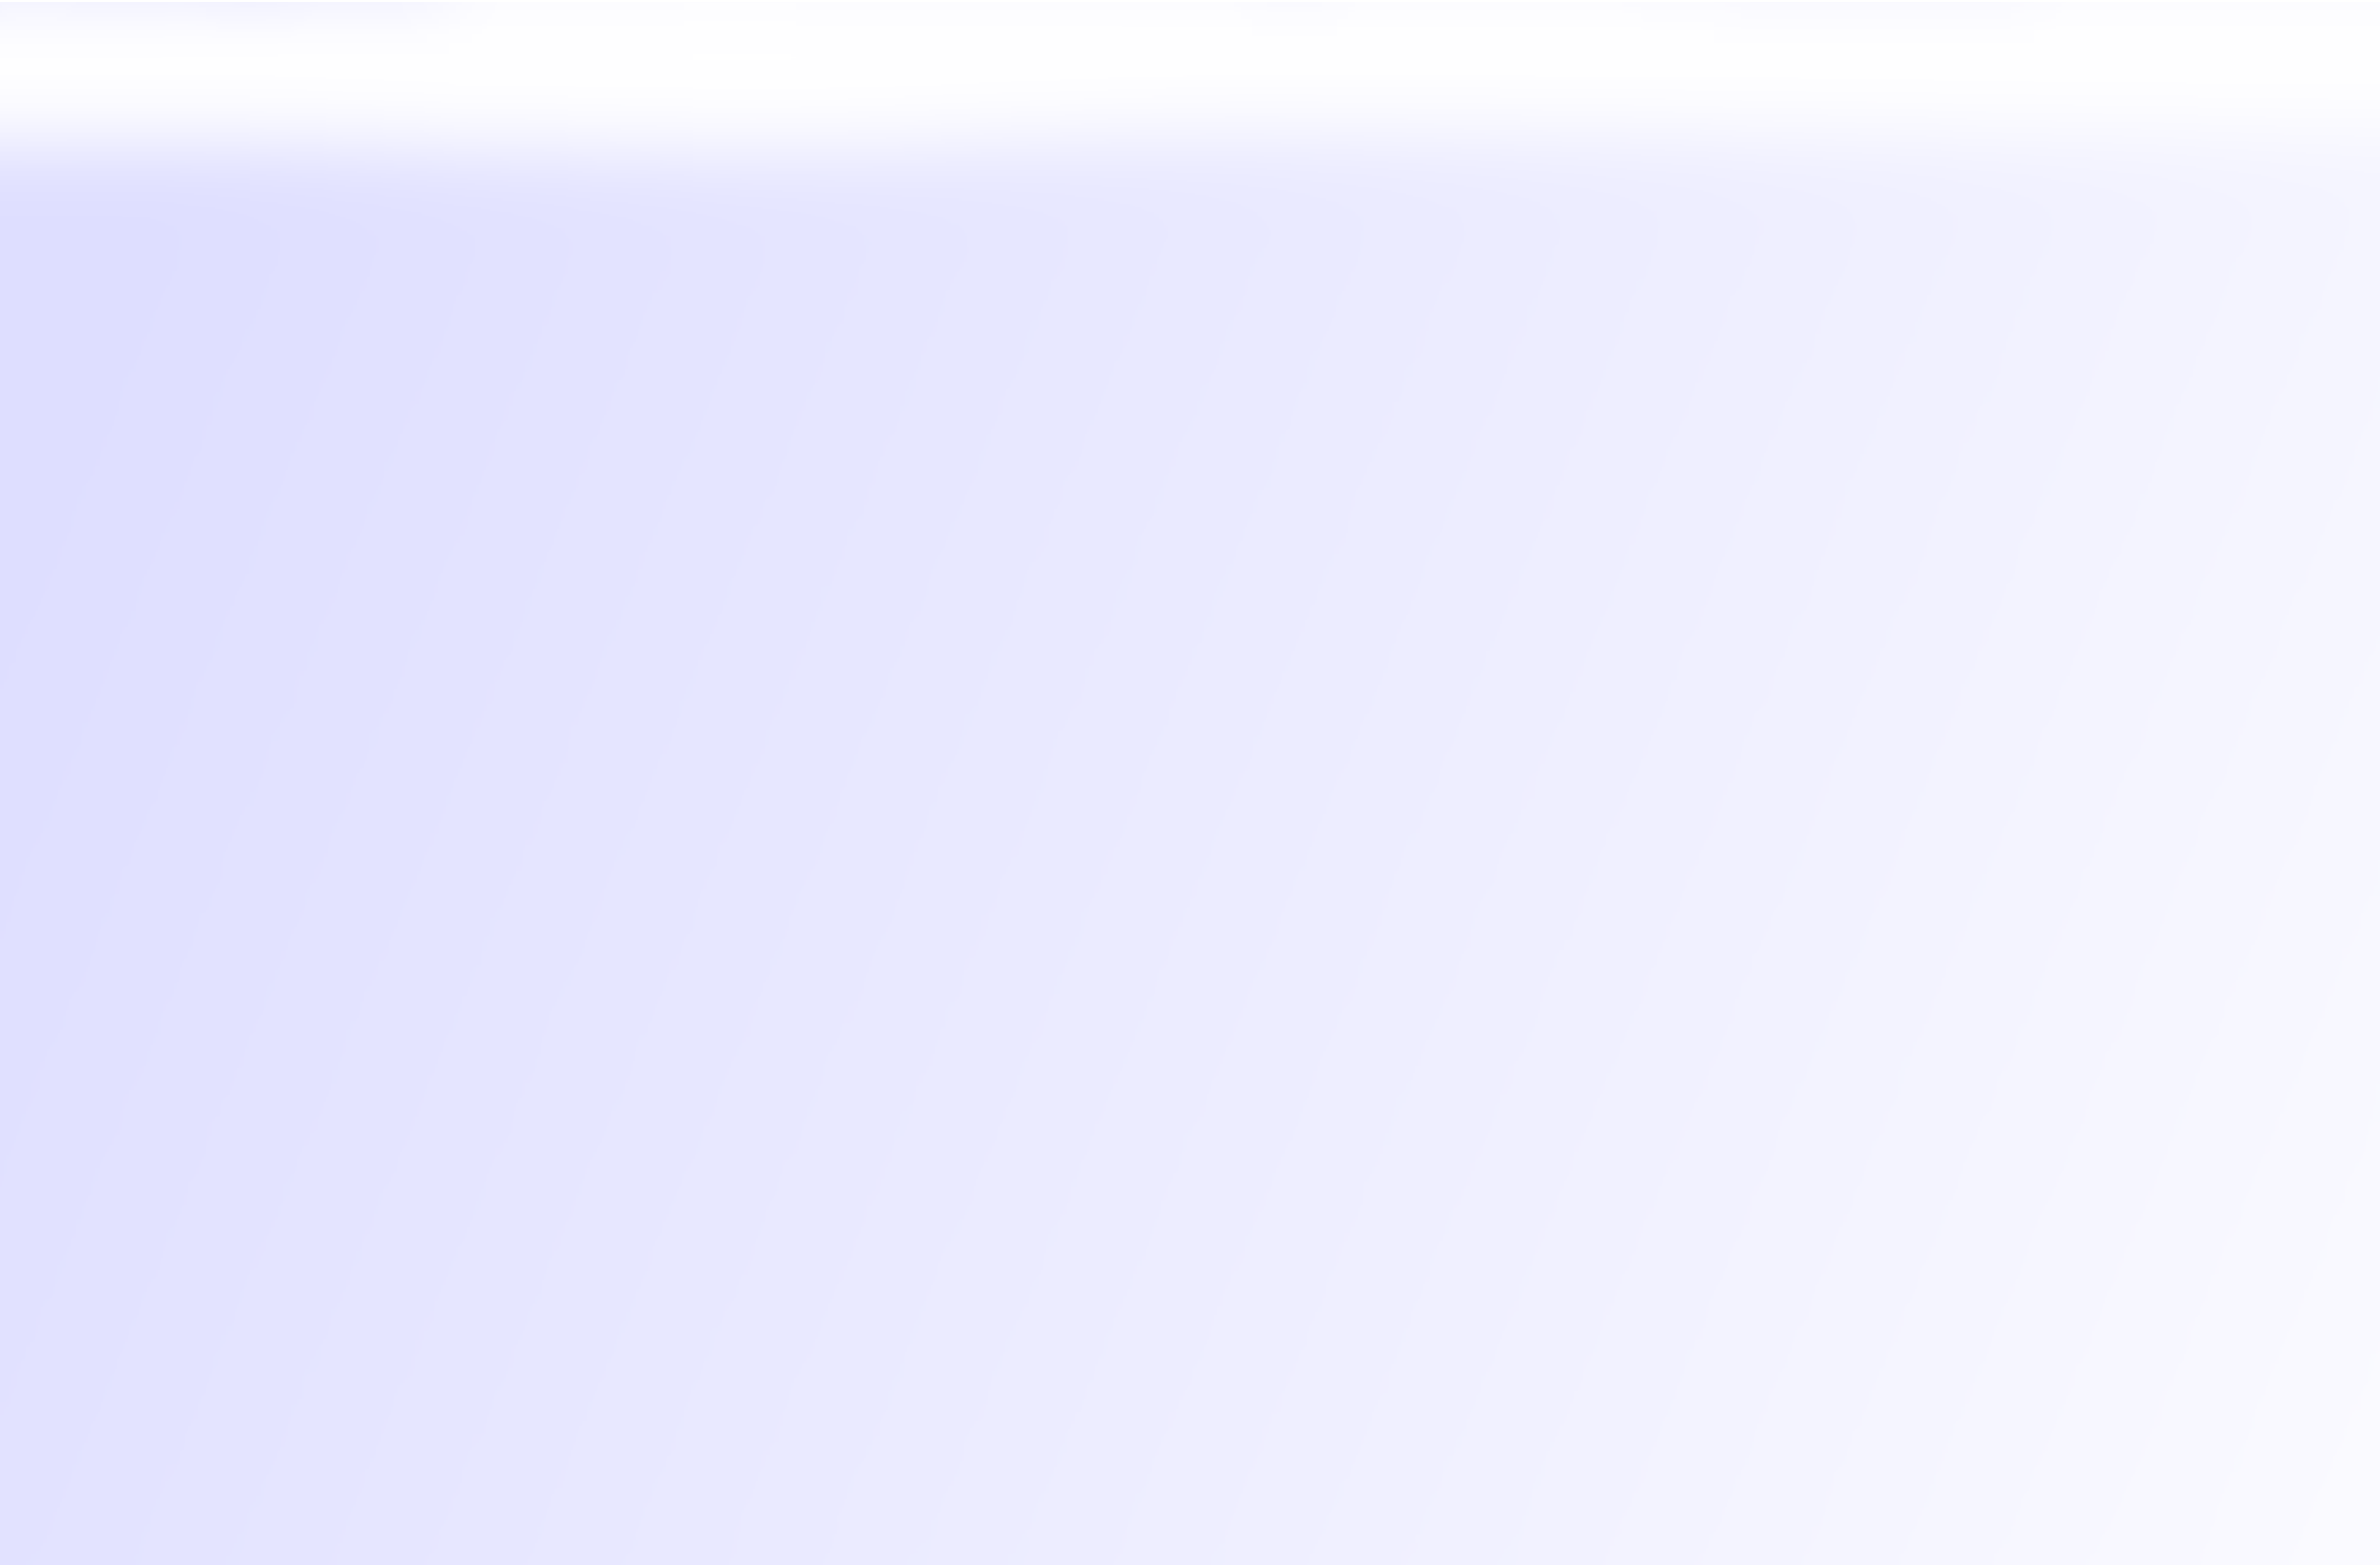
\includegraphics[height=1.1\textheight]{background}};
	%\end{tikzpicture}
}

\begin{poster}{
		grid=false,
		borderColor=bordercol, % Border color of content boxes
		headerColorOne=headercol1, % Background color for the header in the content boxes (left side)
		headerColorTwo=headercol2, % Background color for the header in the content boxes (right side)
		headerFontColor=headerfontcol, % Text color for the header text in the content boxes
		boxColorOne=boxcolor, % Background color for the content in the content boxes
		headershape=roundedright, % Specify the rounded corner in the content box headers
		headerfont=\Large\sf\bf, % Font modifiers for the text in the content box headers
		textborder=rectangle,
		background=user,
		headerborder=open, % Change to closed for a line under the content box headers
		boxshade=plain,
		columns=4
	}
	{
		
\includegraphics[scale=0.3]{figure/scut.pdf}
	}
	%
	%----------------------------------------------------------------------------------------
	%	TITLE AND AUTHOR NAME
	%----------------------------------------------------------------------------------------
	%
	{ \bf  \huge \centering Java程序设计第一次作业} % Poster title
	{\vspace{0.5em}}

	%----------------------------------------------------------------------------------------
	%	INTRODUCTION
	%----------------------------------------------------------------------------------------
	%----------------------------------------------------------------------------------------
	%	Subpart 以子模块的格式组织海报内容,以\headerbox{标题名称title}{配置信息Info}{内容Content}格式书写
	%----------------------------------------------------------------------------------------
	\headerbox{\large 背景}{name=background,column=0,row=0, span=2}{
		随着人工智能技术与产业的发展,智能机器人与人们生活具有越来越密切的联系。在儿童教育陪伴、医疗看护、导览讲解、商场导购等智能机器人应用中,视觉感知与人机交互是关键技术,即机器人通过获取场景中视觉与语音信息,理解用户需求从而更准确提供各种服务。
		\vspace{0.2em}
		%----------------------------------------------------------------------------------------
		%	居中排列图片,其中width:[0,1],1代表图片宽度被设置为Subpart的width,高度自适应,一般取值0.9,0.8
		%----------------------------------------------------------------------------------------
		\begin{center}
			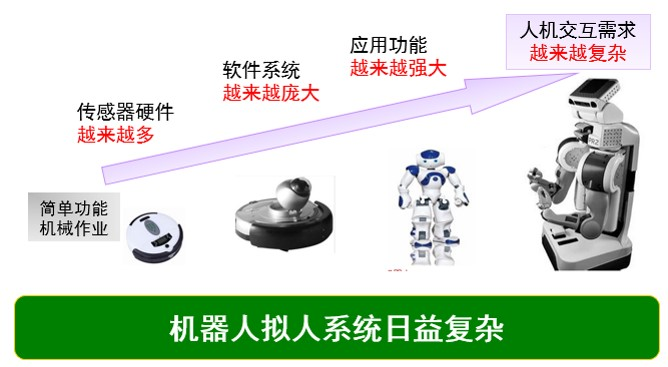
\includegraphics[width=0.9\textwidth]{figure/ex0.jpg}
		\end{center}
		近年来,随着机器视觉感知、语音识别与合成技术的发展,人机交互已经获得很大的进步。智能机器人需求持续增长,未来发展潜力巨大。
		\vspace{0.2em}
	}

	%----------------------------------------------------------------------------------------
	%   Info 配置信息的内容包括: name 模块别名, column 列 默认从0开始代表第一列, row 行 同列, span 边距
	%                             below 在某个模块的下方,定位模式为按照数组索引和相对位置同时定位
	%----------------------------------------------------------------------------------------
	\headerbox{\large 关键研究问题与创新点}{name=main-problem,column=0,row=1, span=2, below=background}{
		\vspace{0.2em}
		%----------------------------------------------------------------------------------------
		%	设置无序列表项。\blue \red是自定义的标签
		%----------------------------------------------------------------------------------------
		\begin{itemize}
			\item
			      \blue{视觉感知}:构建动态的视觉感知与检测模型,在真实环境中检测物体库同步动态更新,提高机器人对环境的信息获取能力与视觉导航精度,提升机器人对环境的适应性
			\item
			      \blue{人机交互}:提升外部感知的多模态信息的智能理解;基于强化学习理论设计对话激励和评价策略,强化人机交互拟人表达能力
			\item
			      \blue{多模态信息理解}:基于累积注意力机制提取多模态信息关键内容,提升机器人对外部感知的信息的智能理解能力
			\item
			      \blue{轻量级模型}:研究通道剪枝的方法压缩深度学习模型,使得算法模型更适合部署至机器人系统上
		\end{itemize}
		\vspace{0.2em}
	}


	\headerbox{\large 研究概况}{name=overview,column=0,row=2, span=2, below=main-problem}{
		\vspace{0.2em}
		首先研究模型剪枝压缩技术以降低深度模型资源要求,围绕多模态信息展开基于累积注意力机制和最优传输理论的信息理解与融合,并基于此实现精准的机器人视觉引导,最后利用强化学习技术寻求更好的交互效果以达到智能机器人系统更为实用的目的。
		\begin{center}
			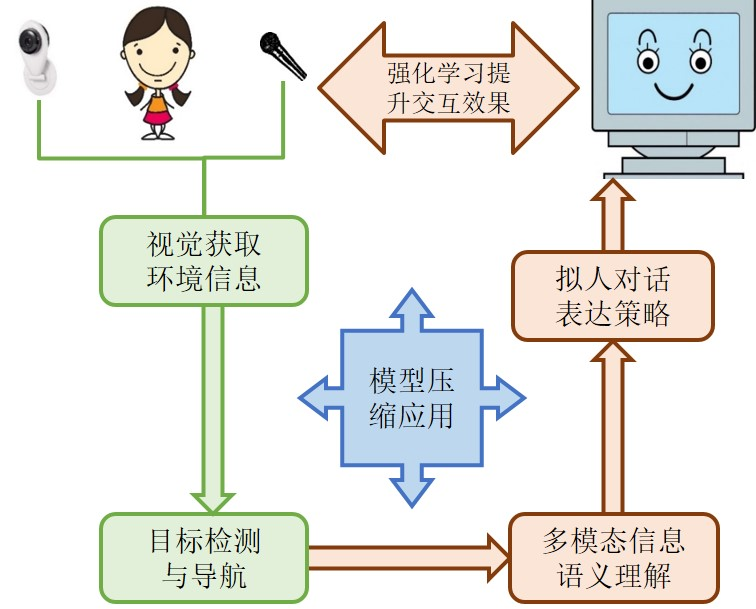
\includegraphics[width=0.813\textwidth]{figure/ex1.jpg}
			\\
			\scriptsize{\label{fig:spot}
				系统研究示意图
			}
		\end{center}
		\vspace{0.20cm}
	}


	\headerbox{\large 视觉感知与导航}{name=research-1,column=2,row=0, span=2}{
		研究机器人场景目标视觉信息的自动获取方法;实现真实环境下的机器人自主视觉导航。
		\vspace{0.2em}
		\begin{itemize}
			\item
			      准确有效地获取场景\blue{视觉信息}是机器人\red{可靠运行}的重要基础
			\item
			      基于视觉的机器人\blue{精准导航}是机器人\red{移动执行任务}的前提
		\end{itemize}
		%----------------------------------------------------------------------------------------
		%	居中排列双图片,其中minipage中的width为0.5,均分width
		%   minipage中的内容和单独设置居中图片时没有区别
		%----------------------------------------------------------------------------------------
		\begin{center}
			\centering
			\begin{minipage}{0.5\textwidth}
				\centering
				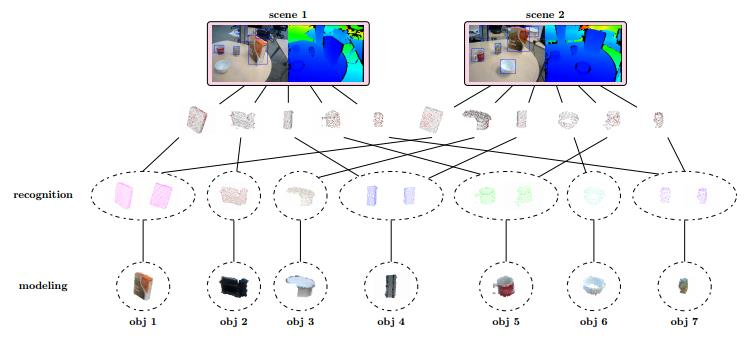
\includegraphics[width=0.9\textwidth]{figure/ex2.jpg}
				\\
				\scriptsize{\label{fig:mug}
					物体识别与模型构建
				}
			\end{minipage}\hfill
			\begin{minipage}{0.5\textwidth}
				\centering
				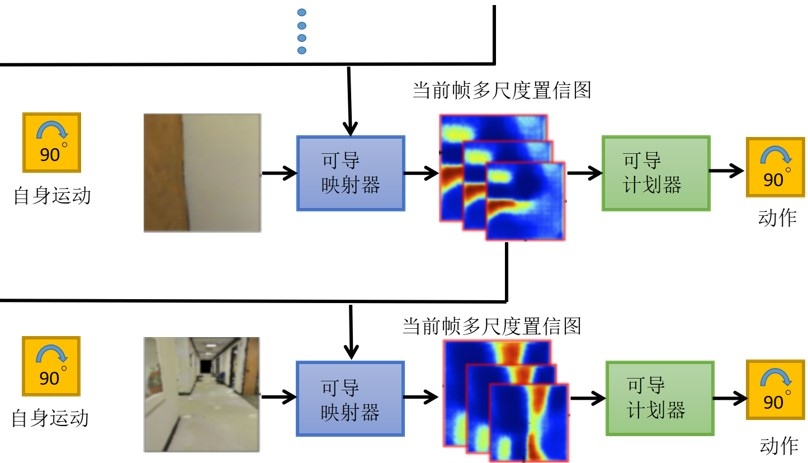
\includegraphics[width=0.9\textwidth]{figure/ex3.jpg}
				\\
				\scriptsize{\label{fig:flood}
					视觉导航
				}
			\end{minipage}
			\\
		\end{center}
		难点:环境中信息复杂多变,识别物体时保证识别效率和准确率;从像素点到动作构建端到端动态导航,保证导航实时性和精准度
		\vspace{0.2em}
	}


	\headerbox{\large 人机交互}{name=research-2,column=2,row=1, span=2, below=research-1}{
		研究多模态智能人机交互技术,包括多模态信息智能理解与多模态拟人表达(语音、文本、动作、表情)实现人机自然交互。
		\begin{itemize}
			\item
			      对外部感知的\blue{多模态信息}进行\red{智能理解与信息融合}让机器人更深地理解真实世界
			\item
			      \blue{自然、高效、友好和智能}地进行人机交互是拟人机器人重要目标
		\end{itemize}
		\begin{center}
			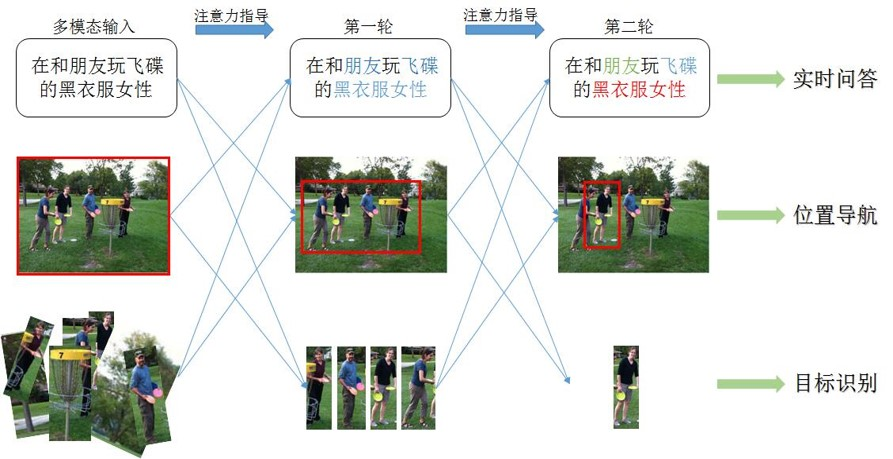
\includegraphics[width=0.8\textwidth]{figure/ex4.jpg}
			\\
			\scriptsize{\label{fig:edges}
				累积注意力机制选取多模态关键信息
			}
		\end{center}
		难点:外部信息存在异构性、复杂性、冗余性,如何对信息进行智能理解获取关键信息;人机交互对话中逻辑、任务、目的需要多样化处理
		\vspace{0.2em}
	}


	\headerbox{\large 轻量级模型压缩}{name=research-3,column=2,row=3, span=2, below=research-2}{
	研究深度模型冗余去除方法,构建高性能的轻量级神经网络模型。
	{\vspace{0.2em}}
	\begin{center}
		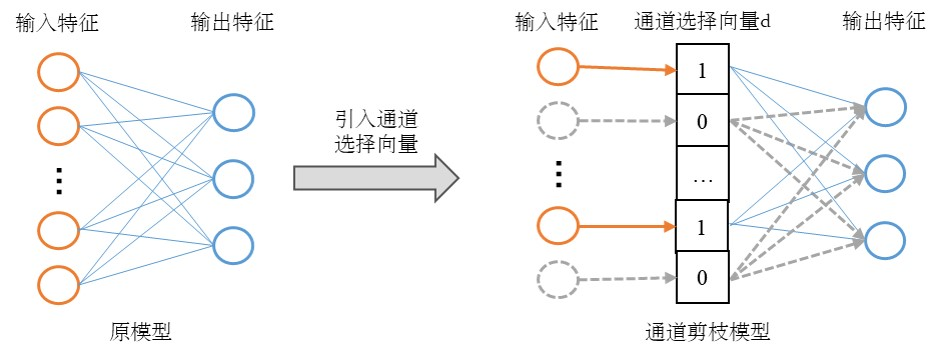
\includegraphics[width=0.8\textwidth]{figure/ex5.jpg}
		\\
		\scriptsize{\label{fig:edges}
			网络层引入选择向量进行模型压缩
		}
	\end{center}
	\vspace{0.2em}
	\begin{itemize}
		\item
		      深度网络模型\blue{精度高}与\red{复杂度高}并存,需要较高的计算硬件支撑,智能机器人设备往往计算资源有限,导致难以部署
		\item
		      将深度网络模型压缩为\blue{轻量级模型}使其便于部署在机器人设备上
	\end{itemize}
	难点:压缩模型以降低复杂度的同时,保障模型的精度效果
	\vspace{0.2em}
	}

\end{poster}
\end{document}
